% This is samplepaper.tex, a sample chapter demonstrating the LLNCS macro
% package for Springer Computer Science proceedings; Version 2.20 of 2017/10/04
%
\documentclass[runningheads]{llncs}
%
\usepackage{graphicx}
% Used for displaying a sample figure. If possible, figure files should be
% included in EPS format.
%
% If you use the hyperref package, please uncomment the following line to
% display URLs in blue roman font according to Springer's eBook style:
% \renewcommand\UrlFont{\color{blue}\rmfamily}

\begin{document}
%
    \title{Web Colaborativa com Braid e CRDTs} 
    \subtitle{Relatório Final da UC de PIIC}
    %
    %\titlerunning{Abbreviated paper title} If the paper title is too long for
    % the running head, you can set an abbreviated paper title here
    %
    \author{João Oliveira\\Orientado por Nuno Preguiça}
    %
    \authorrunning{João Oliveira, sobre orientação de Nuno Preguiça}
    % First names are abbreviated in the running head. If there are more than
    % two authors, 'et al.' is used.
    %
    \institute{DI - Faculdade de Ciências e Tecnologia - Universidade Nova de
        Lisboa \email{jfv.oliveira@campus.fct.unl.pt}}
    %
    \maketitle              % typeset the header of the contribution
    %
    \begin{abstract}
        Neste relatório é apresentado o trabalho feito ao longo da unidade
        curricular de PIIC-ADC. Começando por uma apresentação do tema em
        questão

        \keywords{First keyword, Second keyword, Another keyword.}
    \end{abstract}
    %
    %
    % o que este trabalho trata?
    \section{Introdução}

        % o que é a web colaborativa? (introdução ao tema)
        \subsection{Colaboração e Aplicações {\itshape Web} Colaborativas}

        Geralmente, a colaboração é definida como o processo de duas ou mais
        pessoas, entidades ou organizações trabalharem em conjunto para
        completar uma tarefa ou atingir um objetivo \cite{collab-def}. 
        
        Já no contexto da informática e dos sistemas distribuidos, uma das
        primeiras aparições do termo surgiu em 1991, com a definição de
        {\itshape groupware} ({\itshape group} + {\itshape software}) por Ellis
        et al.: "Especificamente, definimos groupware como: sistemas baseados em
        computadores que suportam grupos de pessoas envolvidas numa tarefa (ou
        objetivo) e que fornecem uma interface para um ambiente
        partilhado"\cite{groupware-def}. 

        Nos dias de hoje, o {\itshape groupware} assume uma forma
        indiscutivelmente diferente desde a sua genesis em 1991. Devido à sua
        popularidade e abrangência, a {\itshape web} e os dispositivos moveis
        são os mercados alvo da maioria das empresas produtoras de software.
        Devido a isto, vemos serviços de {\itshape groupware} a aparecer mais
        neste tipo de meios. Como exemplo temos serviços como o Google Docs,
        Google Slides, Trello, WhatsApp, Twitter, Facebook e muitos mais a serem
        criados todos os dias. 

        A característica que destingue as aplicações {\itshape web}
        colaborativas de outras aplicações {\itshape web} é o facto de existir a
        noção de um estado partilhado para o qual os utilizadores contribuem com
        um objetivo ou propósito em vista. Pegando no exemplo do Facebook, o
        propósito pode ser a troca de ideias e impressões nos comentários de uma
        publicação, no caso geral, ou a divulgação de um produto no {\itshape
        Facebook Marketplace}, por parte de um comerciante.

        % porque é que isto é releavante? (apresentação leitor<->tema)
        % \subsection{Popularidade das Aplicações {\itshape Web} Colabrativas}

        % Na realidade, dentro das aplicações {\itshape web} as aplicações
        % {\itshape web} colaborativas são de longe das mais usadas e que motivam
        % mais pessoas a usar a {\itshape web}.

        % Em 2021, 57\%\cite{eurostat-soc-media-usage} da população europeia já
        % usou redes sociais. No mesmo ano, nos EUA, os valores apontam para tão
        % alto quanto 70\%\cite{usa-soc-media-usage}. Já no oriente, os número não
        % ficam muito aquém, com a China e a India com valores\footnote{É
        % importante notar que o relatório citado usa o número de utilizadores
        % bruto, ou seja, não filtra utilizadores falsos ou duplicados. Não
        %obstante disso, com estas figuras podemos concluir que as redes sociais
        %são consideravelmente populares no oriente, visto o valor obtido para a
        % India ser o mais baixo desta região e representar por volta de 1/3 da
        % população.} de 68\% e 34\%, respetivamente\cite{digital2022}.

        % A popularidade destas aplicações é inegável. Esta popularidade devesse,
        % em larga escala, à tecnologia que as suporta e que introduz
        % funcionalidades críticas para a experiência de utilização. 

        % introdução aos CRDTs

        \subsection{{\itshape CRDT}s}

        No que toca à experiência de utilização, um dos focos no desenho de
        aplicações {\itshape web} colaborativas é que trabalhar no ambiente
        colaborativo da aplicação se assemelhe, tanto quanto possível, a
        trabalhar num ambiente colaborativo tradicional. Logo, a componente de
        sincronização de dados é das mais importantes no desenho do sistema
        distribuído que suporta a aplicação. 

        Os "Tipos de dados Replicados sem Conflito", habitualmente denominados
        {\itshape CRDT}s (do inglês {\itshape Conflict Free Replicated Data
        Type}s), são abstrações de tipos de dados desenhadas para permitirem a
        replicação de dados por múltiplos processos com coordenação assíncrona,
        através da troca de mensagens entre as réplicas e de métodos
        determinísticos\cite{CRDTs}. De uma forma mais geral, os {\itshape
        CRDT}s garantem acesso aos dados localmente, com modificações ao seu
        estado a serem propagadas a outras réplicas de forma assíncrona e não
        necessariamente sequencial.

        Assim, num sistema distribuido, os {\itshape CRDT}s garantem alta
        disponibilidade no acesso a dados replicados, consistência e tolerância
        a falhas de rede. Isto vem tornar a tecnologia dos {\itshape CRDT}s cada
        vez mais atrativa, nomeadamente no desenho de um sistema que suporta
        aplicações {\itshape web}, havendo soluções que fazem uso destes tipos
        abstratos de dados tanto no {\itshape backend} como no {\itshape
        frontend} das aplicações.

        % a.k.a: o que é que esta treta toda tem a ver com o trabalho?
        \subsection{Problemas de {\itshape standardização} e o Protolo Braid}
        
        Os protocolos 

        No entanto, no caso das aplicações {\itshape web} colaborativas, em que
        é essencial a sincronização, a {\itshape standardização} dos protocolos
        de comunicação fica áquem. 
        
        A falta de um protocolo de sincronização geralmente aceite leva a que as
        soluções de sincronização recorram a modelos de comunicação {\itshape
        ad-hoc}, tal como comunicação por eventos\footnote{Por exemplo {\itshape
        socket.io} ou {\itshape web-socket}s} ou técnicas como {\itshape
        long-polling}. 

        

            % apresentação do Braid

            \subsubsection{Braid:} Como resposta a este problema da falta de
            estandardização, têm aparecido de comunidades como a "Braid", que
            imaginam um futuro em que as aplicações comunicam de uma forma clara
            e coesa, através de um único protocolo, permitindo integração nativa
            com outras aplicações.

            Mais concretamente, a comunidade Braid está a desenvolver um
            protocolo no contexto da IETF, convenientemente chamado Braid. 

            Segundo o {\itshape draft} para a IETF, o protocolo Braid é "um
            conjunto de extensões que generalizam o protocolo HTTP de um
            protocolo de transferência de estado para um protocolo de
            sincronização de estado [...] colocando o poder de OT e dos CRDTs na
            web, melhorando a performance de rede e permitindo aplicações web
            serem nativamente P2P, colaborativamente editáveis e {\itshape
            offline-first}"\cite{braid-spec}. 


        \paragraph{Sample Heading (Fourth Level)}
        The contribution should contain no more than four levels of headings.
        Table~\ref{tab1} gives a summary of all heading levels.

        \begin{table}
        \caption{Table captions should be placed above the tables.}\label{tab1}
        \begin{tabular}{|l|l|l|}
        \hline
        Heading level &  Example & Font size and style\\
        \hline
        Title (centered) &  {\Large\bfseries Lecture Notes} & 14 point, bold\\
        1st-level heading &  {\large\bfseries 1 Introduction} & 12 point, bold\\
        2nd-level heading & {\bfseries 2.1 Printing Area} & 10 point, bold\\
        3rd-level heading & {\bfseries Run-in Heading in Bold.} Text follows &
        10 point, bold\\
        4th-level heading & {\itshape Lowest Level Heading.} Text follows & 10
        point, italic\\
        \hline
        \end{tabular}
        \end{table}


        \noindent Displayed equations are centered and set on a separate line.F
        \begin{equation}
        x + y = z
        \end{equation}
        Please try to avoid rasterized images for line-art diagrams and schemas.
        Whenever possible, use vector graphics instead (see Fig.~\ref{fig1}).

        %\begin{figure} 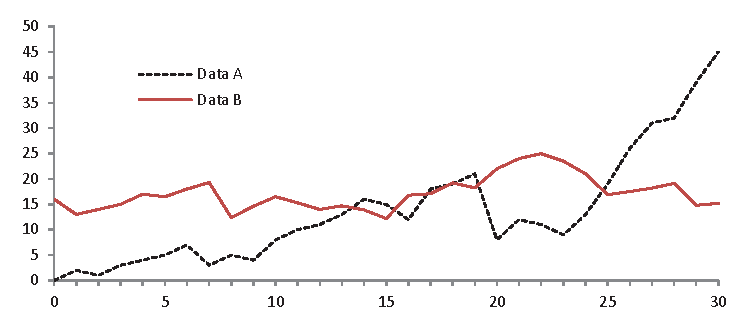
\includegraphics[width=\textwidth]{fig1.eps} \caption{A
        %figure caption is always placed below the illustration. Please note
        %that short captions are centered, while long ones are justified by the
        %macro package automatically.} \label{fig1} \end{figure}

        \begin{theorem}
        This is a sample theorem. The run-in heading is set in bold, while the
        following text appears in italics. Definitions, lemmas, propositions,
        and corollaries are styled the same way.
        \end{theorem}
        %
        % the environments 'definition', 'lemma', 'proposition', 'corollary',
        % 'remark', and 'example' are defined in the LLNCS documentclass as
        % well.
        %
        \begin{proof}
        Proofs, examples, and remarks have the initial word in italics, while
        the following text appears in normal font.
        \end{proof}
        For citations of references, we prefer the use of square brackets and
        consecutive numbers. Citations using labels or the author/year
        convention are also acceptable. The following bibliography provides a
        sample reference list with entries for journal
        articles~\cite{ref_article1}, an LNCS chapter~\cite{ref_lncs1}, a
        book~\cite{ref_book1}, proceedings without editors~\cite{ref_proc1}, and
        a homepage~\cite{ref_url1}. Multiple citations are grouped
        \cite{ref_article1,ref_lncs1,ref_book1},
        \cite{ref_article1,ref_book1,ref_proc1,ref_url1}.
    %
    % ---- Bibliography ----
    %
    % BibTeX users should specify bibliography style 'splncs04'. References will
    % then be sorted and formatted in the correct style.
    %
    % \bibliographystyle{splncs04} \bibliography{mybibliography}
    %

    \bibliographystyle{splncs04}
    \bibliography{refs}

    %\begin{thebibliography}{3}

    %\bibitem{CRDTs} Shapiro, M., Preguiça, N., Baquero, C., Zawirski, M.:
    %Conflict-free replicated data types. In 13th international conference on
    %Stabilization, safety, and security of distributed systems (SSS'11), pp.
    %386–400 Springer-Verlag, Berlin, Heidelberg. 

    %\bibitem{groupware-def}

    %\bibitem{braid-spec} It is inappropriate to use Internet-Drafts as
    %reference material or to cite them other than as "work in progress."

    %\bibitem{collab-def} Marinez-Moyano, I. J. Exploring the Dynamics of
    %Collaboration in Interorganizational Settings, Ch. 4, p. 83, in Schuman
    %(Editor). Jossey-bass, 2006. ISBN 0-7879-8116-8.

    %\bibitem{digital2022}

    %\bibitem{eurostat-soc-media-usage}

    %\bibitem{usa-soc-media-usage}

    %\end{thebibliography}
\end{document}
